\chapter{Obsah CD}
\begin{itemize}
    \item doc/ -- složka s dokumentací (vygenerováno nástrojem Doxygen).
    \item src/ -- složka se zdrojovými kódy.
	\begin{itemize}
	    \item core/ -- složka se zdrojovými kódy jádra knihovny.
	    \item include/ -- složka s hlavičkovými soubory jádra.
	    \item modules/ -- složka se zdrojovými kódy modulů.
	    \item README -- manuál k zprovoznění a spuštění nástroje.
	\end{itemize}
    \item text/ -- složka se zdrojovými kódy technické zprávy.
    \item Doxygen -- soubor s konfigurací doxygenu.
    \item estimate\_time.py -- slouží k výpočtu času potřebného k prolomení uvedeného hesla při
	uvedené rychlosti.
    \item LICENSE -- text licence MIT.
    \item README -- základní info s obsahem CD a seznamem změn oproti původní verzi.
    \item obnova\_hesel\_archivu\_zip\_s\_vyuzitim\_GPU.pdf -- elektronická verze této technické zprávy.
\end{itemize}
\chapter{Typy GPU generátorů}
\label{CPUGPU}
\begin{figure}[ht]
    \begin{center}
	\scalebox{0.25}{
	    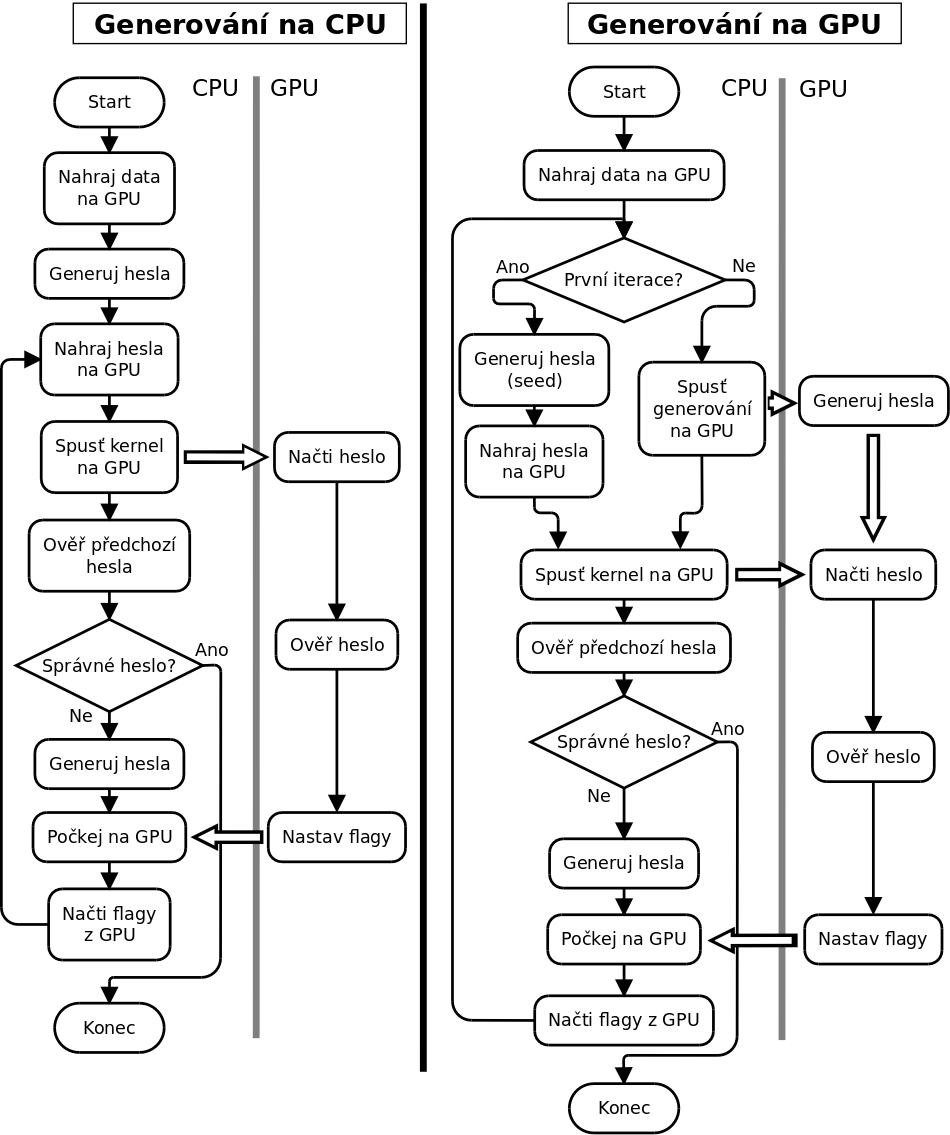
\includegraphics{fig/generators}
	}
    \end{center}
    \caption{Proces generování hesel na CPU a~ověřování na GPU vlevo. Generování a~ověřování na
	GPU vpravo. \cite{Schmied}}
\end{figure}
%\chapter{Manual}
%\chapter{Konfigrační soubor}
%\chapter{RelaxNG Schéma konfiguračního soboru}
%\chapter{Plakat}

